\begin{abstract}
% 问题背景和难点：说明 UOT 的作用以及无熵离散问题的规模瓶颈。
Unbalanced optimal transport (UOT) compares distributions while allowing their total mass to vary, yet its discrete formulation still involves quadratically many transport variables.
% 我们的主要思路
Exploiting the existence of sparse optimal couplings, we develop \ours, which combines a GPU-friendly first-order solver, \subsolver, with dynamic active-support updates to solve large-scale UOT in linear memory.
% CN: 突出反复非线性受限求解的瓶颈及 PDUOT 的作用。
% EN: Highlight repeated nonlinear restricted solves and the role of PDUOT.
Within this alternating process, \subsolver efficiently handles the nonlinear restricted UOT subproblems, computing high-accuracy couplings and dual potentials that guide subsequent support updates.
% CN: 分别陈述内层收敛与非精确受限求解下的外层有限终止。
% EN: State inner convergence and finite outer termination with inexact restricted solves.
Theoretically, we establish global convergence and a local linear rate for \subsolver, whose stopping rules ensure finite termination of \ours's support refinement to a prescribed KKT tolerance despite inexact restricted solves.
% CN: 以扩展及规模、效率和下游任务证据收口。
% EN: Close with extensions and evidence on scale, efficiency and downstream tasks.
We further extend the method to sparse entropic UOT and unbalanced fused Gromov--Wasserstein problems.
Experiments demonstrate efficient scaling to million-point problems on a single GPU and broad applicability across ground costs, marginal penalty types, and penalty strengths.
Downstream evaluations on biological alignment tasks further show substantial speedups with competitive task performance.
\end{abstract}

\section{Introduction}

Optimal transport (OT) provides a geometric framework for comparing distributions and aligning datasets, while unbalanced optimal transport (UOT) relaxes marginal constraints to allow mass variation~\citep{chizat2018scaling,sejourne2023unbalanced}.\setcounter{footnote}{1}\footnote{The source code is available at {\def\UrlBreaks{\do\/}\url{https://anonymous.4open.science/r/Salut-F0F2/}}.}
% CN: 先介绍单细胞应用，再列举其他领域及其需要边际放松的原因。
% EN: Introduce single-cell applications first, followed by other fields and their motivations for marginal relaxation.
This flexibility supports applications in single-cell genomics~\citep{schiebinger2019optimal,klein2025mapping}, domain adaptation~\citep{fatras2021unbalanced}, and point-cloud motion estimation~\citep{puy2020flot}, accommodating cell proliferation and death, mismatched class proportions, and occlusions.

Let $\mathbf{a}\in\mathbb R_{++}^m$ and $\mathbf{b}\in\mathbb R_{++}^n$ be the reference masses of two discrete measures, and let $\mathbf{C}\in\mathbb R^{m\times n}$ be their pairwise cost matrix.
UOT minimizes transport cost plus divergence penalties on the deviations of the transported marginals from $\mathbf{a}$ and $\mathbf{b}$.
% \xwz{The general-marginal-penalty appendix is temporarily omitted; restore its cross-reference only after that extension is written.}
We mainly focus on the widely used KL marginal penalties:
\begin{equation}
\label{eq:primal-uot}
\min_{\mathbf{X}\geq 0}\quad \langle \mathbf{C},\mathbf{X}\rangle+\rho_a\KL(\mathbf{X}\mathbf{1}_n\,|\,\mathbf{a})
+\rho_b\KL(\mathbf{X}^\top\mathbf{1}_m\,|\,\mathbf{b}),
\end{equation}
Here, $\mathbf{X}\in\mathbb R_+^{m\times n}$ is the coupling, $\rho_a,\rho_b>0$ control the marginal penalties, and $\KL(\mathbf{p}\,|\,\mathbf{h})=\sum_k(p_k\log(p_k/h_k)-p_k+h_k)$.
For $\ell_2^2$ marginal penalties, Appendix~\ref{app:l2-penalty} provides corresponding convergence guarantees, with experiments in Appendix~\ref{app:l2-experiments}.

The dual of~\eqref{eq:primal-uot} optimizes potentials $\mathbf{f}\in\mathbb R^m$ and $\mathbf{g}\in\mathbb R^n$:
\begin{equation} 
\label{eq:dual-uot}
\begin{aligned}
&D(\mathbf{f},\mathbf{g}):=\rho_a\langle \mathbf{a},\mathbf{1}_m-e^{-\mathbf{f}/\rho_a}\rangle
+\rho_b\langle \mathbf{b},\mathbf{1}_n-e^{-\mathbf{g}/\rho_b}\rangle,\\
&\max_{\mathbf{f},\mathbf{g}}D(\mathbf{f},\mathbf{g})\quad\text{s.t.}\quad f_i+g_j\leq C_{ij}\quad\forall i,j.
\end{aligned}
\end{equation}
The primal formulation has one transport variable for each of the $mn$ source--target pairs; the dual has only $m+n$ potentials but still imposes $mn$ constraints.
This quadratic problem size poses substantial memory and computational challenges at large sample sizes.

\paragraph{Related work.}
Regularization methods add penalties to the transport plan to facilitate optimization, including $\ell_2^2$ regularization~\citep{nguyen2023unbalanced} and, most prominently, entropic regularization.
The latter enables generalized \sinkhorn iterations, including stabilized and translation-invariant scaling variants~\citep{chizat2018scaling,schmitzer2019stabilized,pham2020unbalanced,sejourne2022faster}.
However, additional regularization introduces bias relative to unregularized UOT, and entropic regularization generally yields a dense coupling whose explicit materialization requires $\Theta(mn)$ memory.

Low-rank methods constrain the coupling to admit a compact nonnegative factorization, improving computational and memory scalability at a fixed rank~\citep{scetbon2023unbalanced,halmos2024low}.
This scalability comes at the cost of potentially substantial approximation error when the chosen rank is insufficient to represent the optimal coupling.

Several methods target the original UOT objective directly, including multiplicative coupling updates (\mm)~\citep{chapel2021unbalanced}, marginal-first reformulations (\etm)~\citep{liu2026solving}, and Frank--Wolfe reductions such as \hellouot~\citep{sejourne2022faster,xia2026dual}.
However, standard \mm implementations store the full coupling; \etm requires Sinkhorn-type $O(mn)$ updates for marginal estimation; and \hellouot repeatedly invokes balanced OT oracles.
% Another approach exploits coupling sparsity through a network-simplex framework that maintains forest-supported transport plans~\citep{agazzotti2026network}.
% Scalability remains limited by quadratic coupling storage in standard \mm implementations, the cost of marginal estimation or sequential balanced OT subproblems in reduction methods, and sequential tree updates in network simplex that hinder GPU parallelization.
% This leaves open how to solve the large scale unregularized UOT problem with linear memory and efficient GPU parallelism.

Existing methods that exploit coupling sparsity face different limitations: regularization paths require quadratic marginal penalties~\citep{chapel2021unbalanced}; 
network simplex relies on sequential tree updates that complicate GPU parallelization~\citep{agazzotti2026network}; 
safe screening provides no linear-memory guarantee throughout optimization~\citep{su2025safe}; 
and cost truncation lacks numerical validation~\citep{auricchio2026transport}.
This leaves open how to solve large-scale UOT problems with linear memory and efficient GPU parallelism.

\paragraph{Our approach.}
UOT admits sparse optimal couplings, motivating optimization over a small active support.
We introduce \ours, a \textbf{S}calable \textbf{A}lgorithm for solving \textbf{L}arge-scale \textbf{U}O\textbf{T} in linear memory.
It alternates optimization on the active support with support updates to identify missing transport variables.

A central computational bottleneck is the repeated solution of nonlinear restricted UOT subproblems.
To address this bottleneck, we develop \subsolver, a GPU-efficient first-order primal--dual solver that returns both the coupling and dual potentials for subsequent support updates.
We establish convergence guarantees for its adaptive iteration and design stopping rules that ensure finite support refinement to a prescribed KKT tolerance with inexact restricted solves.
Following \hello's dual-guided hierarchy~\citep{xia2026dual}, we use dual potentials from smaller problems to initialize the active support and dual violations to guide support updates.
To guarantee linear working memory, we combine budgeted pruning with support sparsification that preserves both transported marginals and transport cost.

Our contributions are summarized as follows:
\begin{itemize}
    \item \textit{GPU-efficient restricted solver:} We develop \subsolver, a GPU-friendly first-order primal--dual solver for nonlinear restricted UOT subproblems.
It efficiently computes high-accuracy solutions across a wide range of marginal penalty strengths.
    \item \textit{Large-scale UOT with linear memory:} Building on \subsolver, we develop \ours, which combines restricted UOT solves with dynamic active-support management to solve large-scale UOT in linear memory.
Experiments demonstrate million-point scalability on a single GPU and applicability across costs and marginal penalty types.
   \item \textit{Convergence guarantees:} We establish global convergence and a local linear rate for the full \subsolver algorithm.
    Its stopping rules further ensure that \ours's support refinement reaches a prescribed full-space KKT tolerance in finitely many rounds despite inexact restricted solves.
    \item \textit{Extensions and applications:} We extend \ours to approximate entropic UOT and solve unbalanced fused Gromov--Wasserstein (UFGW) problems, with large-scale biological experiments showing substantial speedups and competitive downstream performance.
\end{itemize}

\section{Scaling UOT with Linear Memory}
\label{sec:method}

\subsection{Method Overview}
\label{sec:framework}

With the transported marginals $\mathbf{X}\mathbf{1}_n$ and $\mathbf{X}^\top\mathbf{1}_m$ fixed, the marginal penalties are constant and minimizing over $\mathbf{X}$ reduces to balanced OT.
Consequently, whenever an optimum exists, there is an optimal coupling with at most $m+n-1$ positive entries.
On an active support $\mathcal N\subseteq[m]\times[n]$, the restricted primal--dual pair is
\begin{equation}
\label{eq:restricted-uot}
\begin{aligned}
\min_{\mathbf X\geq0}\Phi(\mathbf X)\quad&\text{s.t.}\quad \supp(\mathbf X)\subseteq\mathcal N,\\
\max_{\mathbf f,\mathbf g}D(\mathbf f,\mathbf g)
\quad&\text{s.t.}\quad f_i+g_j\leq C_{ij},\quad(i,j)\in\mathcal N,
\end{aligned}
\end{equation}
where $\Phi$ and $D$ are the objectives in~\eqref{eq:primal-uot} and~\eqref{eq:dual-uot}, respectively.

The potentials returned by a restricted solve define the dual score
\begin{equation}
\label{eq:dual-score}
\sigma_{ij}:=f_i+g_j-C_{ij}.
\end{equation}
A positive omitted score identifies a violated dual constraint and provides a candidate for support expansion.
If every omitted score is nonpositive at an exact restricted primal--dual solution, the full KKT conditions hold and that solution is globally optimal (Appendix~\ref{app:refinement-convergence}).
Inspired by column generation for linear programming~\citep{lubbecke2005selected}, we alternate between solving restricted UOT subproblems and updating the active support using dual scores.
The algorithm stops when the full-space KKT tolerance is met; Section~\ref{sec:analysis} establishes finite termination under the stated conditions with inexact restricted solves.

Repeated nonlinear restricted UOT solves are a core computational bottleneck of this approach.
We develop \subsolver to efficiently obtain high-accuracy primal--dual solutions across marginal penalty strengths (Section~\ref{sec:pduot}), with the returned potentials also guiding subsequent support updates.

A good initial active support can reduce subsequent work~\citep{schmitzer2016sparse,xia2026memory}, so we construct a coarse-to-fine hierarchy of UOT problems and use smaller-problem solutions for initialization, following \hello~\citep{xia2026dual}.
Budgeted pruning and support sparsification as needed control support size to maintain linear working memory (Section~\ref{sec:analysis}).
Algorithm~\ref{alg:ours} summarizes the resulting method, with levels indexed from $0$, the finest, to $L$, the coarsest, and primal--dual states $\mathcal Z^{(\ell)}=(\mathbf X^{(\ell)},\mathbf f^{(\ell)},\mathbf g^{(\ell)})$.


\begin{algorithm}[t]
\caption{\ours for UOT}
\label{alg:ours}
\begin{algorithmic}[1]
\STATE \textbf{Input:} UOT hierarchy $\{\mathcal P^{(\ell)}\}_{\ell=0}^{L}$, support budgets $\kappa,\gamma,\beta$, and tolerance $\varepsilon$.
\STATE \textbf{Output:} finest-level primal--dual state $\mathcal Z^{(0)}$.
\medskip
\STATE $\mathcal Z^{(L)}\gets\subsolver(\mathcal P^{(L)},[m_L]\times[n_L],\varnothing;\varepsilon)$
\FOR{$\ell=L-1,\ldots,0$}
    \STATE $\mathcal B\gets\nw(\mathcal P^{(\ell)})$
    \STATE $(\mathcal N,\mathcal Z)\gets\init(\mathcal P^{(\ell)},\mathcal Z^{(\ell+1)},\mathcal B;\kappa)$
    \LOOP
        \STATE $\mathcal Z\gets\subsolver(\mathcal P^{(\ell)},\mathcal N,\mathcal Z;\varepsilon)$
        \STATE $\mathcal Z\gets\sparsify(\mathcal Z)$
        \STATE \textbf{if} $\kkt(\mathcal P^{(\ell)},\mathcal Z)\leq\varepsilon$ \textbf{then break}
        \STATE $\mathcal V\gets\pricing(\mathcal P^{(\ell)},\mathcal Z;\gamma)$
        \STATE $\mathcal N\gets\prune(\mathcal N\cup\mathcal V,\mathcal Z,\mathcal B,\mathcal V;\beta)$
    \ENDLOOP
    \STATE $\mathcal Z^{(\ell)}\gets\mathcal Z$
\ENDFOR
\medskip
\STATE \textbf{Return:} $\mathcal Z^{(0)}$.
\end{algorithmic}
\end{algorithm}

\begin{figure}[t]
\centering
% CN: 手绘概览图源码位于 figures/salut_overview_source；正文载入浏览器导出的 PDF。
% EN: Whiteboard overview sources live in figures/salut_overview_source; include the browser-exported PDF.
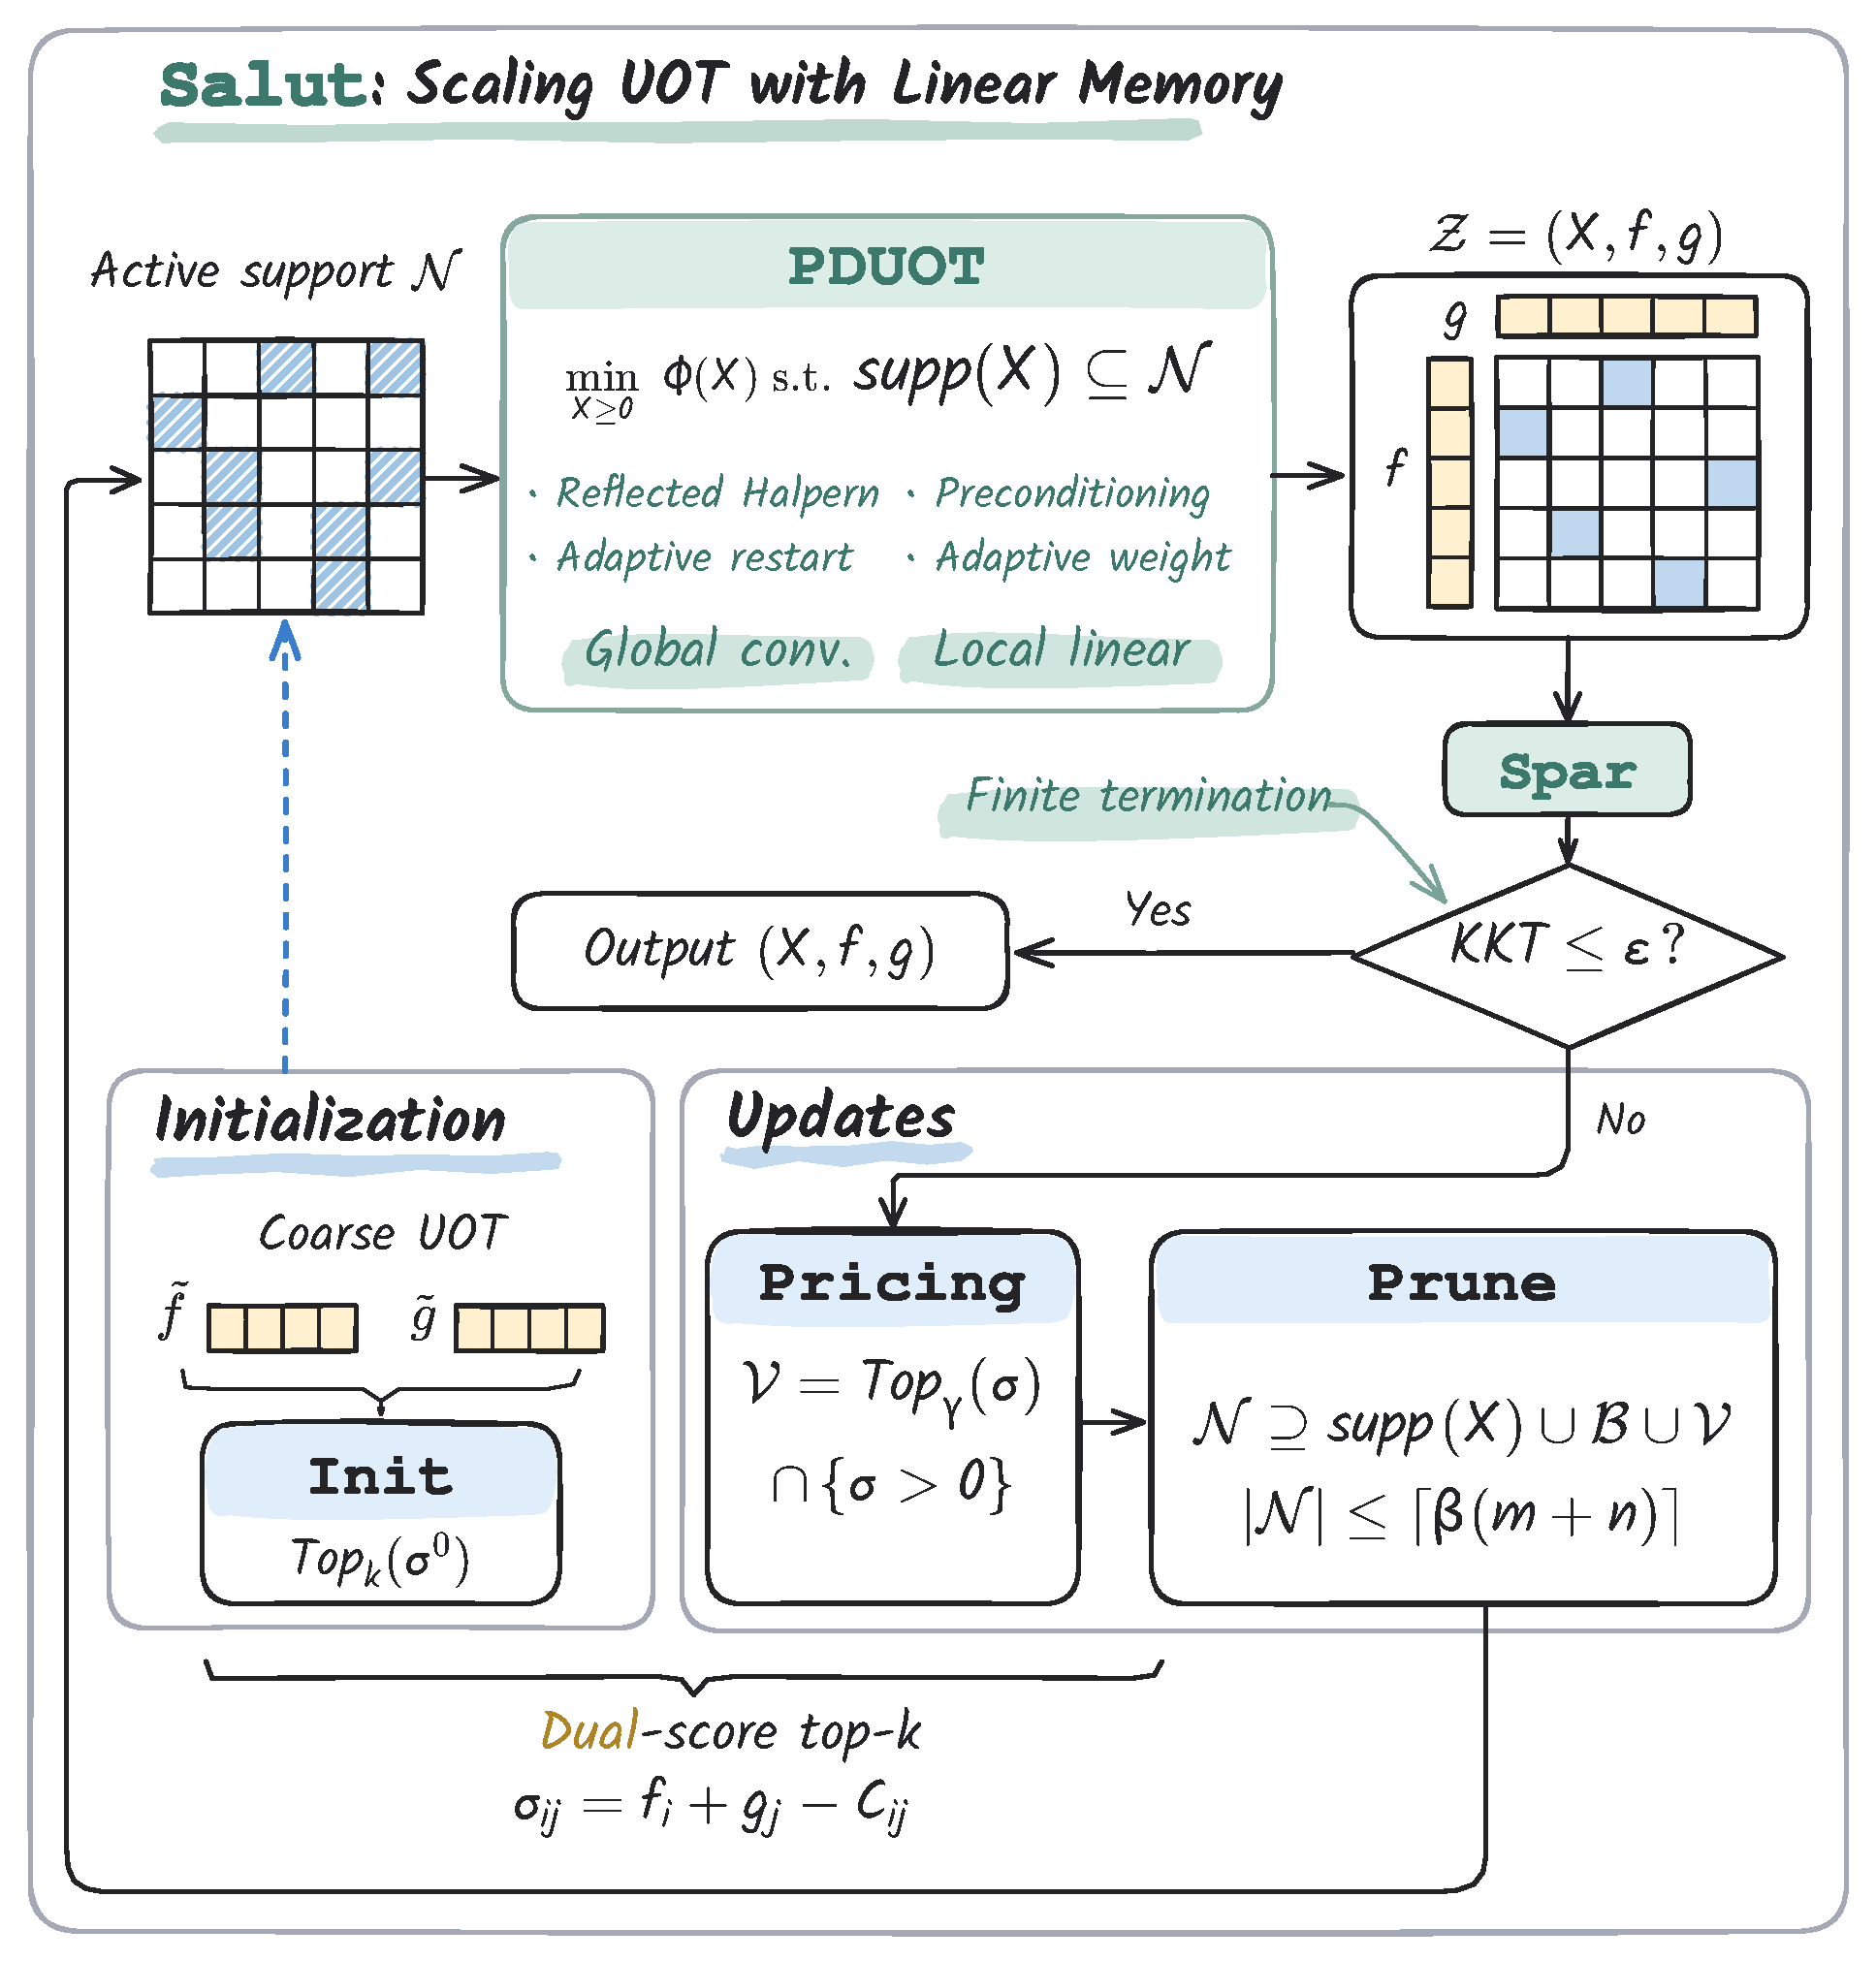
\includegraphics[width=\columnwidth]{figures/salut_overview_whiteboard.pdf}
\caption{\textbf{Overview of \ours.}
Restricted UOT solves with \subsolver alternate with active-support updates, initialized from a coarser UOT solution.
}
\label{fig:shuttle-overview}
\end{figure}

\subsection{Restricted UOT with \subsolver}
\label{sec:pduot}

For an active support $\mathcal N$, let $\mathbf x\in\mathbb R_+^{|\mathcal N|}$ collect its edge flows and $\mathbf c_{\mathcal N}\in\mathbb R^{|\mathcal N|}$ their costs.
The marginal-sum operator $\mathbf A_{\mathcal N}\in\mathbb R^{(m+n)\times|\mathcal N|}$ satisfies $\mathbf A_{\mathcal N}\mathbf x=(\mathbf X\mathbf1_n,\mathbf X^\top\mathbf1_m)$, where $\mathbf X\in\mathbb R_+^{m\times n}$ is zero outside $\mathcal N$.
With $G(\mathbf r,\mathbf q)=\rho_a\KL(\mathbf r\,|\,\mathbf a)+\rho_b\KL(\mathbf q\,|\,\mathbf b)$, problem~\eqref{eq:restricted-uot} becomes

\begin{equation}
\label{eq:restricted-uot-vector}
\min_{\mathbf{x}\geq0}\;\langle \mathbf{c}_{\mathcal{N}},\mathbf{x}\rangle+G(\mathbf{A}_{\mathcal N}\mathbf{x}).
\end{equation}

We build \subsolver on primal--dual hybrid gradient (PDHG) updates~\citep{esser2010general,chambolle2011first}.
Writing $F(\mathbf x)=\langle\mathbf c_{\mathcal N},\mathbf x\rangle+\iota_{\mathbb R_+^{|\mathcal N|}}(\mathbf x)$ and $\mathbf y=-(\mathbf f,\mathbf g)$ gives the saddle formulation
\begin{equation*}
\min_{\mathbf{x}}\max_{\mathbf{y}}\;F(\mathbf{x})+\langle \mathbf{A}_{\mathcal N}\mathbf{x},\mathbf{y}\rangle-G^*(\mathbf{y}),
\end{equation*}
where
\begin{equation*}
G^*(\mathbf{y})=\rho_a\sum_i a_i(e^{y_i/\rho_a}-1)+\rho_b\sum_j b_j(e^{y_{m+j}/\rho_b}-1).
\end{equation*}

With positive diagonal steps $\mathbf D_x,\mathbf D_y$, the primal-first PDHG map is $\pduotmap(\mathbf x,\mathbf y)=(\widehat{\mathbf x},\widehat{\mathbf y})$:
\begin{equation}
\label{eq:pduot-map}
\begin{aligned}
\widehat{\mathbf{x}}&=\left[\mathbf{x}-\mathbf{D}_x(\mathbf{c}_{\mathcal{N}}+\mathbf{A}_{\mathcal N}^\top \mathbf{y})\right]_+,\\
\widehat{\mathbf{y}}&=\operatorname{prox}_{G^*}^{\mathbf{D}_y^{-1}}\left(\mathbf{y}+\mathbf{D}_y\mathbf{A}_{\mathcal N}(2\widehat{\mathbf{x}}-\mathbf{x})\right).
\end{aligned}
\end{equation} 
The edgewise primal projection and nodewise dual proximal map enable sparse GPU-parallel updates.

\paragraph{Reflected Halpern iteration.}
Following \citet{lu2024restarted,lin2025practical}, we use the reflected Halpern update
\begin{equation*}
\mathbf z^{k+1}
=\frac{\mathbf z^{\mathrm a}+(k+1)(2T\mathbf z^k-\mathbf z^k)}{k+2},
\end{equation*}
where $\mathbf z=(\mathbf x,\mathbf y)$, $\mathbf z^{\mathrm a}$ is the fixed epoch anchor, and $k$ counts iterations within the epoch.

\paragraph{Adaptive restart.}
Following \citet{lu2025cupdlpx}, we trigger a restart when the fixed-point residual decreases sufficiently from the epoch baseline, increases after moderate reduction, or the epoch exceeds a prescribed length.
See Appendix~\ref{app:pduot-controls} for the detailed criteria. 

\paragraph{Preconditioning.}
We use Pock--Chambolle diagonal preconditioning~\citep{pock2011diagonal} to set the base steps $\overline{\mathbf D}_x,\overline{\mathbf D}_y$.

\paragraph{Adaptive weight.}
A weight $w>0$ balances the primal and dual steps through $\mathbf D_x=w\overline{\mathbf D}_x$ and $\mathbf D_y=\overline{\mathbf D}_y/w$.
At restarts, we adapt $w$ using PID-based weight updates following \citet{lu2025cupdlpx}.
To establish convergence with adaptive weights, we additionally impose a summable budget on log-weight changes (see Appendix~\ref{app:pduot-controls}).

Table~\ref{tab:pduot-theory-coverage} compares theoretical coverage with related solvers~\citep{lu2025cupdlpx,lin2025practical,lu2026cupdqpx}, whose convergence guarantees cover restricted configurations rather than the complete practical solvers.
In contrast, our analysis jointly covers all four components used in \subsolver (Theorem~\ref{prop:pduot-convergence}).
Algorithm~\ref{alg:pduot} gives the complete iteration.

% CN: 理论来源：cuPDLPx 及其基础分析 lu2024restarted；PDCS 定理 1 与算法 2；cuPDQPx 定理 2--3 与第 3 节；本文定理 prop:pduot-convergence。
% EN: Theory sources: cuPDLPx and its foundation lu2024restarted; PDCS Theorem 1 versus Algorithm 2; cuPDQPx Theorems 2--3 versus Section 3; our Theorem prop:pduot-convergence.
\begin{table}[t]
\caption{\textbf{Convergence analysis coverage.}
Coverage by the cited analyses:
$\checkmark$: covered; $\triangle$: covered only in special cases; ---: not covered.}
\label{tab:pduot-theory-coverage}
\centering
\begingroup
\footnotesize
\setlength{\tabcolsep}{2pt}
\begin{tabular*}{\columnwidth}{@{\extracolsep{\fill}}lcccc@{}}
\toprule
Method & \shortstack{Reflected\\Halpern} & Precond. & \shortstack{Adaptive\\restart} & \shortstack{Adaptive\\weight} \\
\midrule
\cupdlpx & $\checkmark$ & $\checkmark$ & $\triangle$ & --- \\
\pdcs & $\checkmark$ & $\checkmark$ & $\triangle$ & --- \\
\cupdqpx & $\checkmark$ & $\checkmark$ & $\triangle$ & --- \\
\textbf{\subsolver} & $\checkmark$ & $\checkmark$ & $\checkmark$ & $\checkmark$ \\
\bottomrule
\end{tabular*}
\endgroup
\end{table}

\begin{algorithm}[t]
\caption{\subsolver for restricted UOT}
\label{alg:pduot}
\begin{algorithmic}[1]
\let\COMMENT\paperalgorithmcomment
\let\algorithmiccomment\paperalgorithmrightcomment
\STATE \textbf{Input:} problem $\mathcal P$, support $\mathcal N$, state $\mathbf z^0$, weight $w_0>0$, tolerance $\varepsilon$.
\STATE \textbf{Output:} coupling $\widehat{\mathbf x}$ and potentials $(\widehat{\mathbf f},\widehat{\mathbf g})$.
\medskip
\STATE $(\overline{\mathbf D}_x,\overline{\mathbf D}_y)\gets\precond(\mathbf A_{\mathcal N})$ \COMMENT{Preconditioning}
\STATE $\mathbf z^{\mathrm a}\gets\mathbf z^0$, $w\gets w_0$, $j\gets0$, $\mathcal H\gets\varnothing$
\LOOP
    \STATE $\mathbf D_x\gets w\overline{\mathbf D}_x$, $\mathbf D_y\gets\overline{\mathbf D}_y/w$
    \STATE $\mathbf z\gets\mathbf z^{\mathrm a}$, $k\gets0$
    \LOOP
        \STATE $(\widehat{\mathbf z},\boldsymbol\lambda,r)\gets\pdhg(\mathbf z;\mathbf D_x,\mathbf D_y)$
        \STATE \textbf{if} $\checkstop(\widehat{\mathbf z},\boldsymbol\lambda;\varepsilon)$ \textbf{then return} $(\widehat{\mathbf x},-\widehat{\mathbf y})$
        \STATE \textbf{if} $\checkrestart(r;\mathcal H)$ \textbf{then break} \COMMENT{Adaptive restart}
        \STATE $\mathbf z\gets\dfrac{\mathbf z^{\mathrm a}+(k+1)(2\widehat{\mathbf z}-\mathbf z)}{k+2}$\COMMENT{Reflected Halpern}
        \STATE $k\gets k+1$
    \ENDLOOP

    \STATE $j\gets j+1$
    \STATE$w\gets\updateweight(\widehat{\mathbf z},\mathbf z^{\mathrm a},w;j)$\COMMENT{Adaptive weight}
    \STATE $\mathbf z^{\mathrm a}\gets\widehat{\mathbf z}$
\ENDLOOP
\end{algorithmic}
\end{algorithm}

\subsection{Active-Support Initialization and Updates}

At each finer level, we initialize the active support using dual potentials from a coarser UOT solution, then refine the active support while controlling its size.

\paragraph{Active-support initialization.}
For UOT problems sharing one side, changes in that side's normalized optimal marginal-response shape are bounded in terms of the cost interaction relative to its marginal penalty (Proposition~\ref{prop:uot-hierarchy-stability}, Appendix~\ref{app:uot-hierarchy-stability}).
This stability motivates a shared-side hierarchy following \hello~\citep{xia2026dual}, with adjacent levels changing only one side.
We inherit the shared-side potential, complete the other by a $c$-transform, and reconcile the potentially unequal marginal-response totals using the optimal translation of \citet[Proposition~2]{sejourne2022faster}:
\begin{equation*}
(\mathbf f,\mathbf g)\leftarrow(\mathbf f+t^\star\mathbf1_m,\mathbf g-t^\star\mathbf1_n).
\end{equation*}
Here $t^\star$ maximizes the dual objective over scalar shifts, while all dual scores remain unchanged (see Appendix~\ref{app:hierarchy-init}).

The resulting scores $\boldsymbol\sigma^0$ guide active-support initialization: writing $\operatorname{Top}_k(\boldsymbol\sigma)$ for the union of the top-$k$ edges in each row and column, we construct
\begin{equation*}
\mathcal N=\operatorname{Top}_{\kappa}(\boldsymbol\sigma^0)\cup\mathcal B.
\end{equation*}
Here $\mathcal B=\nw(\mathcal P)$ contains the structural edges constructed from the reference weights, which prevent the active support from imposing additional marginal mismatch under strong marginal penalties (see Appendix~\ref{app:structural-mismatch}).

% 历史：c3a9938 恢复并保护 NW；f7e83c6 整理相关诊断。
% 实验记录：paper_experiments/uot/diagnostics_20260920/initial_support_reference.md（2026-09-20，TOME，1024×1024）。
% 后续诊断：主仓库提交 7f4a10a（2026-10-19）；脚本与报告见 experiments/nw_structural_role/。
% TOME 对照中 assignment 已连通且覆盖节点；NW 正流边和本次随机补边均消除 Hall 缺口，零流连接边及永久保护 NW 未显示一致的额外收益。
% rho=1e8 的新快照：零 coupling 配继承势或全零势均达 200k；配核验后的最优势则 9900 次收敛，最优 coupling 配继承势仍达上限。
% 27/29 正流分量产生约 -3.57e6 的相对势偏移，全局 translation 无法修复；大势还放大 split-gap 中的边际误差，高精度重算一致。
% 以上为有限快照上的实验诊断，详见 WARMSTART_RESULTS.md；固定 metric 的 Hall 下界另存于 theory/notes/support_induced_iteration_lower_bound.md，不属于自适应收敛证明。

\paragraph{Active-support updates.}
After each restricted solve, we expand the active support using positive-score candidates selected by the same bidirectional top-$k$ rule:
\begin{equation*}
\mathcal V=\operatorname{Top}_{\gamma}(\boldsymbol\sigma)\cap\{(i,j):\sigma_{ij}>0\}.
\end{equation*}
These candidates are identified by \pricing without storing the full cost matrix (see Appendix~\ref{app:hierarchy-pricing}).

The existence of a sparse optimum does not guarantee that an approximate restricted solution leaves sufficient room for new candidates within the support budget.
When needed, \sparsify mixes two cycle-cancellation outputs with costs bracketing the original cost, yielding at most $2(m+n-1)$ positive entries while preserving both transported marginals and the UOT objective.

Finally, \prune removes the lowest-score edges outside $\supp(\mathbf X)\cup\mathcal B\cup\mathcal V$ until the support budget is met (see Appendix~\ref{app:hierarchy-pruning}).
Together with tiled pricing, this ensures $O(m+n)$ memory for fixed feature dimension and support-budget parameters, as shown in Table~\ref{tab:support-size-bounds}.

\subsection{Convergence Analysis}
\label{sec:analysis}

We establish convergence of \subsolver and finite termination of \ours, accounting for their adaptive controls and stopping rules.


\begin{theorem}[Convergence of \subsolver, informal]
\label{prop:pduot-convergence}
\subsolver with the summable weight-update budget~\eqref{eq:pduot-weight-budget} satisfies:
\begin{itemize}
\item \textbf{Global convergence.}
For arbitrary mapped-point restart times, the iterates and mapped points converge to a restricted KKT point from any initial anchor.
\item \textbf{Local linear convergence.}
With sufficiently frequent residual-reduction checks and refreshed baselines after weight updates, convergence is locally R-linear in PDHG evaluations.
\end{itemize}
\end{theorem}

The summable weight-update budget controls metric variation, while mapped-point restarts preserve a common descent estimate.
Residual-reduction checks further yield local linear convergence; formal statements and proofs appear in Appendices~\ref{app:pduot-global}--\ref{app:pduot-restart}.

With inexact restricted solves, positive dual scores need not imply comparable attainable primal improvement.
We therefore couple restricted stopping with objective decrease and pricing accuracy to establish finite refinement termination.
For refinement round $k$, write $\Delta_k=\Phi(\mathbf X^k)-\Phi(\mathbf X^{k+1})$ and $d_k=\varepsilon_{\mathrm r}^2(1+|\Phi(\mathbf X^k)|)$.
Let $G_k$ denote the maximum coordinate gain over newly added candidates, $v_k$ and $a_k$ the full-space and active-support positive-score maxima, and $\Omega_k$ the one-sided marginal-gradient error (defined in Appendix~\ref{app:refinement-convergence}).

\begin{theorem}[Finite refinement termination, informal]
\label{thm:refinement}
Suppose each restricted call returns in finite time to tolerance $\varepsilon_{\mathrm r}>0$, and consecutive refinement outputs satisfy
\begin{equation*}
\begin{gathered}
\Delta_k\geq G_k/2,\\
\Delta_k\geq d_k
\quad\text{or}\quad
\max\{a_{k+1},\Omega_{k+1}\}\leq v_k/2.
\end{gathered}
\end{equation*}
Then refinement terminates in finitely many rounds at restricted tolerance $\varepsilon_{\mathrm r}$ and any prescribed full-space tolerance $\tau>0$.
\end{theorem}

The \checkstop operator is part of \subsolver's stopping rule and enforces these output conditions, which are attained in finitely many iterations under the restricted-solver assumptions (Proposition~\ref{prop:refinement-stop-attainability}, Appendix~\ref{app:refinement-stop-attainability}).
The proof combines objective decrease with violation contraction: rounds without sufficient decrease either contract the maximum dual violation or ensure a uniformly positive decrease in a subsequent round, as detailed in Appendix~\ref{app:refinement-convergence}.
% \xwz{RERUN IN PROGRESS: historical performance measurements have refinement_forcing_check=False and refinement_progress_check=False. Replace them with supported KL/l2-stationarity measurements using the complete Stop rule, preserving each declared cost policy. Numerical bounds use evaluated costs, with scope specified in the appendix.}


\section{Extensions}
\label{sec:extensions}

We further extend \ours to entropic UOT using sparse active-support and to UFGW by embedding it within block coordinate descent.

\subsection{Sparse Entropic UOT}
\label{sec:entropic-extension}

We approximate entropic UOT with regularization strength $\varepsilon>0$ on a sparse active support $\mathcal N_{\mathrm e}$:
\begin{equation}
\label{eq:sparse-entropic-extension}
\min_{X\geq0,\,\supp(X)\subseteq\mathcal N_{\mathrm e}}\;\Phi(\mathbf{X})+\varepsilon\KL(\mathbf{X}\,|\,\mathbf{a}\otimes \mathbf{b}).
\end{equation}
Using the final solution returned by \ours, we set
\begin{equation*}
\mathcal N_{\mathrm e}=\supp(\mathbf X)\cup\operatorname{Top}_{b_{\mathrm e}}(\boldsymbol\sigma),
\end{equation*}
where the budget $b_{\mathrm e}$ can be chosen automatically to fit the final active-support size (see Appendix~\ref{app:entropic-extension}).
Generalized Sinkhorn updates on this support require $O(|\mathcal N_{\mathrm e}|+m+n)=O(m+n)$ time and memory per iteration and return a sparse coupling for downstream tasks; we call this method \ourssparsink.

\subsection{Unbalanced Fused Gromov--Wasserstein}
\label{sec:ufgw-extension}

We consider UFGW with $\ell_2^2$ structural and feature costs, combining feature matching with alignment of within-dataset relations.
In its two-coupling relaxation~\citep{sejourne2023unbalanced}, fixing $\mathbf Q$ gives the KL-UOT subproblem
\begin{equation*}
\begin{aligned}
\min_{\mathbf P\geq0}\,
\langle\mathbf C^{\mathbf Q},\mathbf P\rangle
+|\mathbf Q|(\rho_a\KL(\mathbf P\mathbf1\,|\,\mathbf a)
+\rho_b\KL(\mathbf P^\top\mathbf1\,|\,\mathbf b)),
\end{aligned}
\end{equation*}
where $|\mathbf Q|=\sum_{kl}Q_{kl}$ and $\mathbf C^{\mathbf Q}$ is the cost induced by $\mathbf Q$ (see Appendix~\ref{app:ufgw-extension}).
Block coordinate descent thus produces a sequence of UOT subproblems, which we solve with \ours or, for the entropic variant, \ourssparsink.
We further evaluate costs implicitly from sparse coupling moments, keeping the overall algorithm's memory linear in the number of points for fixed feature dimensions.

\section{Experiments}
\label{sec:experiments}

We evaluate \ours in terms of unregularized UOT accuracy and scalability, restricted-solver efficiency, component contributions, and extensions to entropic UOT and UFGW.

\paragraph{Setup and metrics.}
% CN: 绘图字号与图例间距统一；固定输入、输出哈希及数据一致性检查见 figures/plot_sources/layout_refresh_20261118.json。
% EN: Unified plot typography and legend spacing; fixed inputs, output hashes and data-preservation checks: figures/plot_sources/layout_refresh_20261118.json.
Unless otherwise specified, experiments use TOME E11.5--E12.5 ($d=30$) with $\ell_2^2$ ground costs on a single NVIDIA A100 GPU.
Our main comparison includes \mm, \sinkhorn, and \hellouot; additional baselines are considered in the appendix.
We use weak, moderate, and strong symmetric penalties, $(\rho_a,\rho_b)=(0.1,0.1),(1,1),(10,10)$, and the asymmetric setting $(0.045,99.995)$ adapted from the moscot temporal benchmark~\citep{klein2025mapping}.
We report solver runtime (\runtime, seconds), peak active GPU memory (\gpumemshort, GiB), and primal accuracy using a shared objective gap (\sharedgap)~\eqref{eq:experimental-shared-gap}.
In runtime--accuracy plots, lines connect parameter settings of the same method.
Unless otherwise specified in Appendices~\ref{app:experiment-metrics} and~\ref{app:task-protocols}, results are averaged over five random seeds.
See Appendices~\ref{app:benchmark-data}, \ref{app:implementation-details}, and~\ref{app:experiment-metrics} for dataset and solve details.
% \xwz{RERUN IN PROGRESS: current main-scaling, Pareto, component-ablation, sensitivity, and HELLO-UOT-comparison historical hier_uot batches have refinement_forcing_check=False. Replace their tables/figures with measurements using the complete Stop rule. Preserve the declared cost policy, including coarse FP32 costs.}
% \xwz{Experimental protocol to finalize: hardware, precision, timing and peak-memory measurement, shared-bound construction and validation, parameter grids, and random seeds.
% Exclude compilation warm-up and common accuracy evaluation from solver timing, and disclose their costs separately.}

\subsection{UOT Solver Comparison}
\label{sec:uot-comparison}

\paragraph{Runtime, accuracy, and memory.}
% CN: 定量比较来自 figures/plot_sources/pareto_comparison_analysis_20261119.json；同精度取各方法达到目标 mean gap 的最快扫描点，同预算取不超过基线耗时的 Salut 最小 mean gap，不插值。
% EN: Quantitative comparisons: figures/plot_sources/pareto_comparison_analysis_20261119.json; matched accuracy uses the fastest scanned point meeting the target mean gap, and matched budgets use the smallest Salut mean gap within the baseline runtime, without interpolation.
Figure~\ref{fig:uot-runtime-accuracy} compares \ours with strong UOT baselines. It shows one to three orders of magnitude speedups at comparable accuracy and roughly four to five orders of magnitude smaller gaps within matched runtime budgets.
\ours uses only $0.55$ GiB, versus $16.10$ GiB for \sinkhorn and $56.02$ GiB for \mm, reflecting its linear-memory design.
With each method's representative parameter setting fixed, mean runtimes vary by $3.4\times$ for \ours ($1.66$--$5.62$ seconds), versus $93.5\times$ for \mm, $16.6\times$ for \hellouot, and $21.8\times$ for \sinkhorn across penalty settings, indicating more stable runtime performance across marginal penalty strengths.
\begin{figure}[t]
\centering
% CN: 固定结果及单项正常超时补测见 figures/plot_sources/pareto_final_20261119.json；有效曲线点不变。
% EN: Pinned results and the normal-timeout rerun: figures/plot_sources/pareto_final_20261119.json; valid plotted points are unchanged.
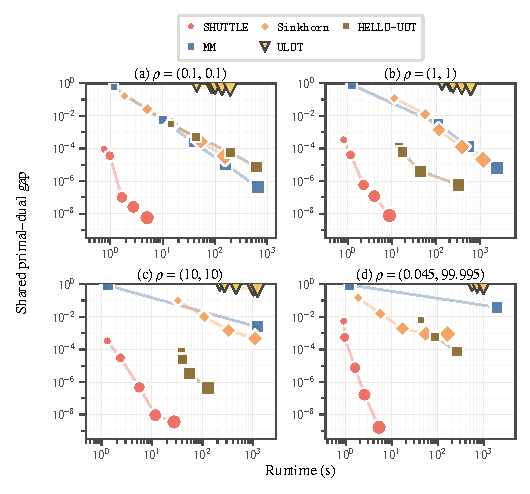
\includegraphics[width=\linewidth]{figures/uot_accuracy_runtime_pareto_2x2.pdf}
\caption{\textbf{Runtime--accuracy comparison.}
$m=n=32{,}768$.
Larger markers target higher accuracy.
The top strip reports the maximum mean peak active GPU memory averaged across plotted configurations and penalty settings.
Protocol in Appendix~\ref{app:uot-comparison-protocol}.
}
\label{fig:uot-runtime-accuracy}
\end{figure}

\paragraph{Comparison with \hellouot.} 
\hellouot scales well and reaches high accuracy faster than other baselines in most penalty settings, but requires repeated balanced-OT oracle calls.
\ours instead solves restricted UOT subproblems directly.
As shown in Table~\ref{tab:hello-uot-main}, at $m=n=131{,}072$, \ours is roughly two orders of magnitude faster than \hellouot at the default inner tolerance while attaining a smaller mean \sharedgap; the same trend holds at $n=65{,}536$ (see Appendix~\ref{app:hello-uot-comparison} for the protocol and trajectories).

\begin{table}[t]
\centering
% CN: 四组 penalty、五 seed 的均值来自 accuracy_runtime_pareto/results/20261119_hello_tolerance_table/summary.json；固定数据见 figures/plot_sources/hello_tolerance_table_20261120.json。
% EN: Means over four penalty settings and five seeds: accuracy_runtime_pareto/results/20261119_hello_tolerance_table/summary.json; pinned data: figures/plot_sources/hello_tolerance_table_20261120.json.
\caption{\textbf{Direct UOT versus balanced-OT reduction.}
Mean over four penalty settings and five random seeds.
The \hellouot rows sweep its inner tolerance, with outer tolerance $100\times$ the inner value; \ours uses tolerance $10^{-6}$.}
\label{tab:hello-uot-main}
\footnotesize
\setlength{\tabcolsep}{2pt}
\begin{tabular*}{\columnwidth}{@{\extracolsep{\fill}}lrrrr@{}}
\toprule
\multirow{2}{*}{Variant} & \multicolumn{2}{c}{$n=65{,}536$} & \multicolumn{2}{c}{$n=131{,}072$} \\
\cmidrule(lr){2-3}\cmidrule(lr){4-5}
& \runtime~$\downarrow$ & \sharedgap~$\downarrow$ & \runtime~$\downarrow$ & \sharedgap~$\downarrow$ \\
\midrule
\hellouot{}\textsubscript{$10^{-4}$} & 38.1 & $2.4\times10^{-3}$ & 122.5 & $2.2\times10^{-3}$ \\
\hellouot{}\textsubscript{$10^{-5}$} & 79.3 & $3.1\times10^{-4}$ & 209.0 & $2.9\times10^{-4}$ \\
\hellouot{}\textsubscript{$10^{-6}$} & 229.3 & $4.7\times10^{-5}$ & 545.8 & $4.8\times10^{-5}$ \\
\ours & \textbf{4.5} & $\boldsymbol{1.1\times10^{-5}}$ & \textbf{7.4} & $\boldsymbol{4.1\times10^{-5}}$ \\
\bottomrule
\end{tabular*}
\end{table}

\paragraph{Scaling to millions with linear memory.}

\begin{figure}[t]
\centering
% CN: 五 seed 图和统计来自 main_scaling/results/20261119_clean_scaling_v2/（15 个计时离群点已在原 batch 上 repair）；100/100 求解及 reference 有效，固定数据见 figures/plot_sources/scaling_final_20261119.json。
% EN: Five-seed plot and statistics: main_scaling/results/20261119_clean_scaling_v2/ (15 timing outliers repaired in place); all 100 solves and references are valid; pinned data: figures/plot_sources/scaling_final_20261119.json.
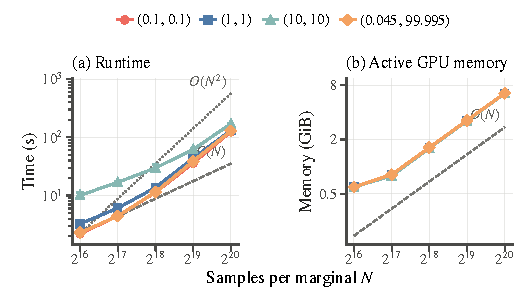
\includegraphics[width=\linewidth]{figures/uot_zhuang_scaling.pdf}
\caption{\textbf{Million-point UOT scalability.}
(a) Runtime and (b) peak GPU memory on Zhuang-ABCA-1$\to$Zhuang-ABCA-2 ($m=n$, $d=30$).
Gray lines indicate linear and quadratic scaling.}
\label{fig:uot-large-scale}
\end{figure}

\begin{table}[t]
\centering
% CN: 假数据占位！仅用于预览排版效果：Online Sinkhorn、ULOT、HELLO-UOT 三行的数值均为猜测的假数据，待百万规模 1 小时上限实测完成后替换。Salut 一行使用 scaling_final_20261119.json 在 n=1,048,576 上四组 penalty、五 seed 的真实均值。
% EN: PLACEHOLDER / MOCK DATA! For layout preview only: the Online Sinkhorn, ULOT, and HELLO-UOT rows contain guessed placeholder numbers to be replaced after running the million-scale one-hour benchmark. The Salut row uses the measured mean over four penalty settings and five seeds at n=1,048,576 from scaling_final_20261119.json.
\caption{\textbf{Million-point comparison against linear-memory baselines} ($m=n=1{,}048{,}576$, Zhuang-ABCA-1$\to$Zhuang-ABCA-2, mean over four penalty settings).
Baselines use a one-hour ($3600$\,s) wall-clock budget ($\varepsilon=10^{-3}$ for online \sinkhorn, rank $128$ for \ulot, inner tolerance $10^{-6}$ for \hellouot); $^\dagger$ indicates hitting the time limit before convergence.}
\label{tab:million-scale-baselines}
\footnotesize
\setlength{\tabcolsep}{2pt}
\begin{tabular*}{\columnwidth}{@{\extracolsep{\fill}}lrr@{}}
\toprule
Method & \runtime~$\downarrow$ & \sharedgap~$\downarrow$ \\
\midrule
Online \sinkhorn & $3600.0^\dagger$ & $1.84\times10^{-1}$ \\
\ulot & $2145.6^\dagger$ & $6.23\times10^{-2}$ \\
\hellouot & $3600.0^\dagger$ & $8.91\times10^{-3}$ \\
\ours & \textbf{138.8} & $\boldsymbol{2.97\times10^{-5}}$ \\
\bottomrule
\end{tabular*}
\end{table}

Figure~\ref{fig:uot-large-scale} scales \ours to over one million points per marginal on whole-brain MERFISH data~\citep{zhang2023wholebrainmerfish}.
Figure~\ref{fig:uot-large-scale} shows linear memory growth and subquadratic runtime growth over the measured range.
At one million points per marginal, \ours takes $126$--$170$ seconds using at most $6.50$ GiB on a single A100, with shared gaps below $7.1\times10^{-5}$ across all cases.
Under a one-hour wall-clock budget at $m=n=1{,}048{,}576$, Table~\ref{tab:million-scale-baselines} further compares \ours against linear-memory baselines: the baselines either exhaust the time budget or remain orders of magnitude less accurate, whereas \ours reaches a mean gap of $2.97\times10^{-5}$ in $138.8$ seconds.

\paragraph{Generality.}
Furthermore, \ours maintains its runtime and accuracy advantages across ground costs, datasets, dimensions, and reference masses (see Appendix~\ref{app:uot-generality}).

\subsection{Restricted UOT Solvers}
\label{sec:restricted-experiments}
\begin{figure}[t]
\centering
% CN: 实验记录见 EXPERIMENT_PROGRESS.md 的 P01；固定图源与统计见 figures/plot_sources/restricted_solver_cdf_20261117.json。
% EN: Experiment record: EXPERIMENT_PROGRESS.md, P01; pinned sources and statistics: figures/plot_sources/restricted_solver_cdf_20261117.json.
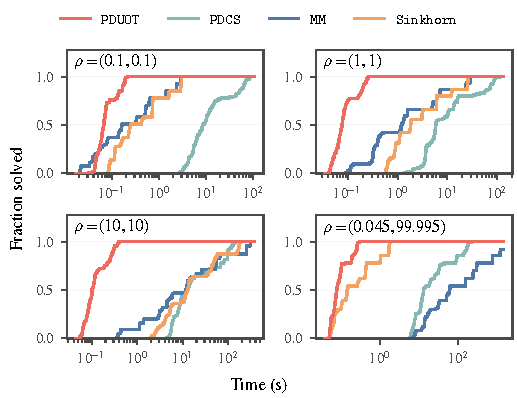
\includegraphics[width=\linewidth]{figures/restricted_solver_runtime_cdf.pdf}
\caption{\textbf{Restricted-solver runtime CDFs.}
Fractions reaching $\sharedgap\leq10^{-4}$ versus runtime on snapshots from \ours runs (parent $m=n=65{,}536$).
Protocol in Appendix~\ref{app:restricted-experiment-protocol}.}
\label{fig:restricted-runtime-cdf}
\end{figure}

Figure~\ref{fig:restricted-runtime-cdf} compares solvers on 433 restricted UOT snapshots captured during \ours runs.
Over same-snapshot pairs reaching the target, \subsolver achieves geometric mean speedups of $153\times$, $40\times$, and $16\times$ over \pdcs, \mm, and \sinkhorn, respectively.
Its mean runtime over successful solves also varies less across penalty settings: $1.7\times$, versus $2.2\times$, $325\times$, and $78\times$ for the respective baselines.
Moreover, \subsolver directly returns primal--dual solutions of the unregularized restricted problem, which \mm and entropic \sinkhorn do not natively provide.


\subsection{Component Analysis}
\label{sec:hierarchy-experiments}

\paragraph{\subsolver components.}
\begin{figure}[t]
\centering
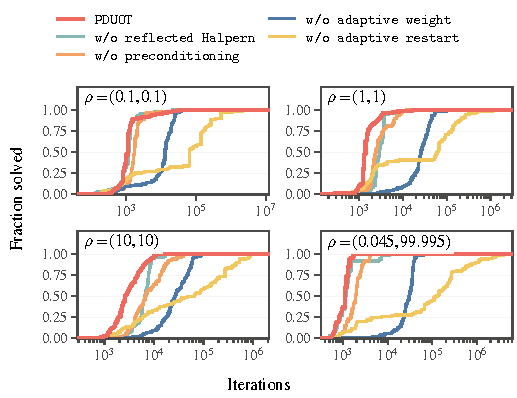
\includegraphics[width=\linewidth]{figures/pduot_component_ablation_cdf_iterations.pdf}
% CN: 实验记录见 EXPERIMENT_PROGRESS.md 的 A04；固定图源与哈希见 figures/plot_sources/pduot_component_ablation_20261117.json。
% EN: Experiment record: EXPERIMENT_PROGRESS.md, A04; pinned sources and hashes: figures/plot_sources/pduot_component_ablation_20261117.json.
\caption{\textbf{Leave-one-out \subsolver component ablations.}
Fractions reaching KKT tolerance $10^{-6}$ versus iterations (one PDHG map evaluation each) on the same snapshots in Figure~\ref{fig:restricted-runtime-cdf}.
Protocol in Appendix~\ref{app:pduot-component-ablation}.}
\label{fig:pduot-component-ablation-cdf}
\end{figure}

Figure~\ref{fig:pduot-component-ablation-cdf} isolates the four components of \subsolver on fixed restricted UOT snapshots.
Adaptive restart and adaptive weight provide the largest reductions in iterations.
Preconditioning reduces mean iterations across all four penalty settings, while reflected Halpern updates help except at the weakest penalty.



\paragraph{\ours components.}

% CN: A--E 分别来自 paper_experiments_uot/component_ablation/results/component_*_5seeds_2026111*/summary_table.json（D 为 translation_n16384_rho1e3_5seeds）；50/50 项方法测量成功，seeds 42--46。
% EN: A--E use paper_experiments_uot/component_ablation/results/component_*_5seeds_2026111*/summary_table.json (D: translation_n16384_rho1e3_5seeds); all 50 method measurements succeed over seeds 42--46.
% CN: 文件哈希、逐 seed 数据、均值和样本标准差固定于 figures/plot_sources/component_ablation_20261120.json；rounds 为 finest_outer_iterations，显存为 peak_gpu_memory_mib / 1024。
% EN: Hashes, per-seed observations, means and sample standard deviations are pinned in figures/plot_sources/component_ablation_20261120.json; rounds are finest_outer_iterations and memory is peak_gpu_memory_mib / 1024.
\begin{table}[t]
\centering
\caption{\textbf{Component ablations.}
$m=n$, KKT tolerance $10^{-6}$.
$n=262{,}144$ for A, $8{,}192$ for B and C, and $16{,}384$ for D and E.
\refineiters counts finest-level refinement rounds.
Protocol in Appendix~\ref{app:system-component-protocol}.
}
\label{tab:component-settings-mock}
\footnotesize
\setlength{\tabcolsep}{1pt}
\renewcommand{\arraystretch}{1.15}
\begin{tabular*}{\columnwidth}{@{\extracolsep{\fill}}llrrr@{}}
\toprule
Component & Variant & \runtime~$\downarrow$ & \refineiters~$\downarrow$ & \gpumemshort~$\downarrow$ \\
\midrule
\multirow{2}{*}{\shortstack[l]{\textbf{A. Hierarchy}\\$\rho=(10,10)$}}
 & \ours & 28.56 & 1.4 & 1.61 \\
 & w/o component & 380.79 & 35.6 & 1.59 \\
\midrule
\multirow{2}{*}{\shortstack[l]{\textbf{B. Active support}\\$\rho=(1,1)$}}
 & \ours & 1.20 & 2.2 & 0.52 \\
 & w/o component & 114.76 & 1.0 & 14.01 \\
\midrule
\multirow{2}{*}{\shortstack[l]{\textbf{C. Solver}\\$\rho=(1,1)$}}
 & \ours & 1.27 & 2.2 & 0.52 \\
 & \ours (\pdcs) & 14.35 & 2.2 & 0.52 \\
\midrule
\multirow{2}{*}{\shortstack[l]{\textbf{D. Translation}\\$\rho=(10^3,10^3)$}}
 & \ours & 12.06 & 5.2 & 0.53 \\
 & w/o component & 28.93 & 5.0 & 0.53 \\
\midrule
\multirow{2}{*}{\shortstack[l]{\textbf{E. Structural edges}\\$\rho=(10^5,10^5)$}}
 & \ours & 9.08 & 5.6 & 0.53 \\
 & w/o component & 44.87 & 7.2 & 0.53 \\
\bottomrule
\end{tabular*}
\end{table}

Table~\ref{tab:component-settings-mock} evaluates components of the complete solver.
The hierarchy reduces mean finest-level refinement from 35.6 to 1.4 rounds and mean runtime by roughly $13\times$, while active-support optimization reduces mean runtime and peak memory by approximately $96\times$ and $27\times$, respectively.
With propagated warm starts for both backends, \subsolver reduces mean runtime by approximately $11\times$ relative to \pdcs.
Removing potential translations and structural edges raises mean runtime by $2.4\times$ and $4.9\times$, respectively.




% CN: 熵正则 UOT、UFGW solver 和下游实验使用实测结果；各图表单独注明来源。
% EN: Entropic UOT, UFGW solver and downstream experiments use measurements, with sources recorded for each figure and table.
\subsection{Extensions}
\label{sec:extension-experiments}
\paragraph{Sparse entropic UOT.}
\label{sec:entropic-experiments}

\begin{figure}[t]
\centering
% CN: 实验记录见 EXPERIMENT_PROGRESS.md 的 Entropic Pareto；固定图源与统计见 figures/plot_sources/entropic_uot_20261117.json。
% EN: Experiment record: EXPERIMENT_PROGRESS.md, Entropic Pareto; pinned sources and statistics: figures/plot_sources/entropic_uot_20261117.json.
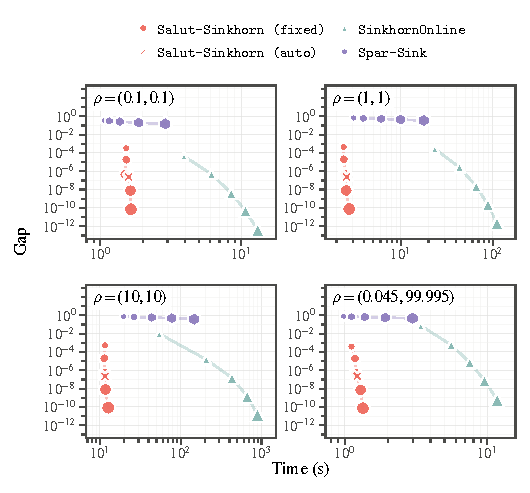
\includegraphics[width=\linewidth]{figures/entropic_uot_accuracy_runtime_pareto_eps0.001.pdf}
\caption{\textbf{Sparse entropic UOT runtime--accuracy comparison.}
$m=n=16{,}384$, $\varepsilon=10^{-3}$.
Larger markers indicate larger budgets or tighter thresholds.
Circles use fixed reconstruction budgets; crosses use automatic budgets.
Protocol in Appendix~\ref{app:extension-protocols}.
}
\label{fig:entropic-runtime-accuracy}
\end{figure}

Figure~\ref{fig:entropic-runtime-accuracy} compares \ourssparsink with online \sinkhorn and \sparsink on the same entropic UOT objective.
Across all four penalty settings, \ourssparsink reaches $\sharedgap<5\times10^{-7}$ in $1$--$12$ seconds at $b_{\mathrm e}=8$, and $\sharedgap<10^{-10}$ at $b_{\mathrm e}=32$.
Appendix~\ref{app:entropic-epsilon-accuracy} further evaluates reconstruction accuracy across entropic strengths.
% \xwz{The unmeasured Schmitzer/LCN appendix and its main-text promise are temporarily omitted.}
% Additional comparisons with Schmitzer's multiscale solver and LCN clustering with sparse \sinkhorn are deferred to Appendix~\ref{app:entropic-additional-baselines}.
% CN: epsilon 扫描来自 paper_experiments_uot/entropic_epsilon_accuracy/results/20261117_paper_data_entropic_epsilon_accuracy/summary.json，140/140成功（五 seed），仅评估返回的 sparse coupling。
% EN: Epsilon-sweep results come from paper_experiments_uot/entropic_epsilon_accuracy/results/20261117_paper_data_entropic_epsilon_accuracy/summary.json, with 140/140 successful five-seed sparse-coupling evaluations.
% \xwz{If warm-start acceleration becomes a central claim, add a main-text comparison of cold-start and hier_uot--Sinkhorn-initialized full Sinkhorn, reporting end-to-end runtime including initialization as well as continuation iterations.}



\paragraph{UFGW.}
\label{sec:ufgw-experiments}

\begin{table}[t]
\centering
% CN: 四行五-seed 实测均值来自 paper_experiments_uot/ufgw_solver_comparison/results/20261117_paper_data_ufgw_solver_comparison/cases/*/{shuttle,pot}_repeat0/metrics.json（seeds 0--4，20/20 成功，含 J=64 与 refinement safeguard）；固定统计与校验和见 figures/plot_sources/ufgw_solver_comparison_20261120.json。
% EN: All four five-seed measured means come from paper_experiments_uot/ufgw_solver_comparison/results/20261117_paper_data_ufgw_solver_comparison/cases/*/{shuttle,pot}_repeat0/metrics.json (seeds 0--4, 20/20 successful ten-sweep runs with J=64 and the refinement safeguard); pinned statistics and checksums: figures/plot_sources/ufgw_solver_comparison_20261120.json.
% CN: Time 使用 runtime_sec；Memory 使用 peak_gpu_memory_mib/1024 转为 GiB；objective 为共同 CPU FP64 目标，含 joint entropy 常数；加速比按未舍入均值耗时计算，不跨 epsilon 比较目标值。
% EN: Time uses runtime_sec; Memory converts peak_gpu_memory_mib to GiB by division by 1024; objectives use the common CPU FP64 evaluator including joint-entropy constants; speedups use unrounded mean times, without comparing objectives across epsilon settings.
% CN: Objective 保留四位小数；同一 epsilon 内按展示精度并列最好的目标值均加粗。
% EN: Objectives are rounded to four decimal places; tied best displayed objectives within each epsilon group are all bolded.
\caption{\textbf{UFGW solver comparison} on STARmap well05--well11 ($m=n=16{,}384$, $d=30$, $\alpha=0.4$, $\rho_a=\rho_b=0.1$).
Each method runs ten complete sweeps from product couplings.
\ufgwobj denotes the two-coupling UFGW objective with entropy strength $\varepsilon$ (Appendix~\ref{app:ufgw-extension}).
Protocol in Appendix~\ref{app:extension-protocols}.
}
\label{tab:ufgw-solvers}
\footnotesize
\setlength{\tabcolsep}{2pt}
\begin{tabular}{@{}clrrr@{}}
\toprule
$\varepsilon$ & Method & \runtime~$\downarrow$ & \gpumemshort~$\downarrow$ & \ufgwobj~$\downarrow$ \\
\midrule
\multirow{2}{*}{$0$} & \bcdmm & 481.53 & 40.02 & 0.1114 \\
 & \oursufgw & \textbf{16.05} & \textbf{0.53} & \textbf{0.1111} \\
\midrule
\multirow{2}{*}{$10^{-3}$} & \bcdsinkhorn & 102.75 & 34.27 & \textbf{0.1223} \\
 & \ourssinkhornufgw & \textbf{17.58} & \textbf{0.53} & \textbf{0.1223} \\
\bottomrule
\end{tabular}

\end{table}


Table~\ref{tab:ufgw-solvers} compares our UFGW extensions with POT's \bcdmm and \bcdsinkhorn on the same two-coupling objective under a common sweep budget.
Our variants are $30.0\times$ and $5.8\times$ faster at $\varepsilon=0$ and $10^{-3}$, respectively, attain lower or comparable objectives, and reduce peak GPU memory by over $98\%$.
Objective--time trajectories appear in Appendix~\ref{app:ufgw-solver-trajectories}.


\subsection{Downstream Applications}
\label{sec:downstream-applications}

\paragraph{Temporal transport.}
% \xwz{RERUN REQUIRED FOR THE WEIGHT-BUDGET CHANGE: the archived hier_uot temporal results do not provide complete per-call restart counts across all time pairs, so unchanged behavior under J=64, p=1.01 cannot be established. Rerun the hier_uot--Sinkhorn configurations and update the linked temporal figures and timing breakdown; keep historical provenance and the authors' per-pair penalties. Full-rank and low-rank baselines are unaffected by this controller change. Audit: experiments/primal_weight_budget_20261111/report/history_J64_audit.json.}
We evaluate temporal transport on 19 adjacent time pairs from the moscot mouse embryogenesis benchmark~\citep{klein2025mapping} in Figure~\ref{fig:temporal-runtime}, using the published per-pair settings.
% CN: 数值来自 paper_experiments_uot/moscot_time/results/20261102_005354_paper_data/{summary.csv,summary_table.csv}，114/114 项已完成；加速比按同一时间对的 coupling_evaluation_sec 相除，含 coupling 与 evaluation。
% EN: Numbers come from paper_experiments_uot/moscot_time/results/20261102_005354_paper_data/{summary.csv,summary_table.csv}, with 114/114 configurations complete; speedups divide paired coupling_evaluation_sec values, including coupling computation and evaluation.
Compared with rank-2000 \ulot~\citep{scetbon2023unbalanced}, \ourssparsink is $4.91$--$17.71\times$ faster, with a mean absolute difference in \transitionacc\ from the full-rank \sinkhorn reference of only $0.21$ percentage points versus $2.03$.
% CN: rank2000 配对加速和 MOSTA 平均准确率提升核验见 figures/plot_sources/downstream_analysis_20261117.json。
% EN: Rank-2000 paired speedups and the MOSTA mean accuracy gain are audited in figures/plot_sources/downstream_analysis_20261117.json.

\begin{figure}[t]
\centering
% CN: 三联图来自 paper_experiments_uot/moscot_time/results/20261102_005354_paper_data/temporal_runtime_accuracy.pdf；数据为同目录 summary.csv、summary_table.csv；114/114 已完成。
% EN: Triptych source: paper_experiments_uot/moscot_time/results/20261102_005354_paper_data/temporal_runtime_accuracy.pdf; data: summary.csv and summary_table.csv in the same batch; 114/114 complete.
% CN: 本次从 figures/plot_sources/experiment_figures_20261114.json 的固定汇总输入重画，入口为 scripts/refresh_experiment_figures.py；图例使用 Salut-Sinkhorn。
% EN: Redrawn from the pinned aggregate inputs in figures/plot_sources/experiment_figures_20261114.json via scripts/refresh_experiment_figures.py, with the Salut-Sinkhorn legend.
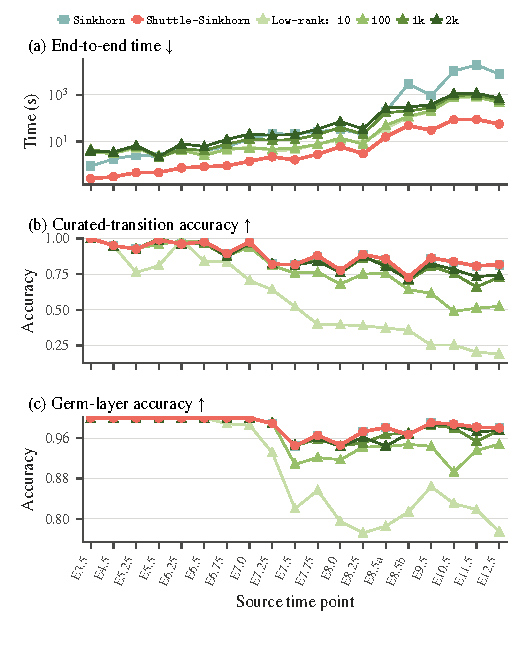
\includegraphics[width=\linewidth]{figures/moscot_time_runtime_accuracy.pdf}
\caption{\textbf{Temporal transport on mouse embryogenesis.}
(a) Coupling computation plus downstream evaluation time; (b) curated transition accuracy; (c) germ-layer accuracy.
Triangle labels denote \ulot ranks ($1\mathrm{k}=1000$).
Each horizontal position denotes a distinct adjacent-time-pair instance; higher accuracy is better.
Protocol in Appendix~\ref{app:downstream-protocol}.}
\label{fig:temporal-runtime}
% \xwz{SEED COVERAGE: Current application plots use seed 42 only; 19 time pairs are distinct tasks, not independent random seeds. Add four seeds and refresh both accuracy and timing figures.}
\label{fig:temporal-accuracy}
\end{figure}

\paragraph{Spatial alignment.}
\begin{table}[t]
\centering
% CN: 两方法实测精度与正式 runtime_sec 均来自 paper_experiments_uot/moscot_spatiotemporal/results/20261101_213655_selected_compare_im2/{summary.csv,summary.json,cases/*/*/metrics.json}，14/14 成功且收敛。BCD 参数来源：results/20261031_203031_my4090/selection.json；ULFGW 使用本次 config.yaml 的作者最优参数。表格四舍五入，加速比按未舍入耗时计算。
% EN: Measured accuracies and formal runtime_sec for both methods come from paper_experiments_uot/moscot_spatiotemporal/results/20261101_213655_selected_compare_im2/{summary.csv,summary.json,cases/*/*/metrics.json}, with 14/14 successful converged runs. BCD parameters: results/20261031_203031_my4090/selection.json; ULFGW uses the author-selected parameters in this measurement batch's config.yaml. Table entries are rounded; speedups use unrounded times.
\caption{\textbf{Spatiotemporal alignment on MOSTA.}
Columns denote seven adjacent-time-pair instances, labeled by source embryonic day (E).
\ours represents \ourssinkhornufgw; \moscot is low-rank UFGW.
\transitionacc\ is in percent; higher is better.
Time excludes downstream evaluation.
Protocol in Appendix~\ref{app:downstream-protocol}.
}
% \xwz{SEED COVERAGE: Current MOSTA table uses seed 0 only across seven time pairs. Add four independent seeds for the selected configurations; time pairs do not count as seeds.}
\label{tab:ufgw-application}
\footnotesize
\setlength{\tabcolsep}{2.3pt}
\renewcommand{\arraystretch}{1.12}
\begin{tabular}{@{}llrrrrrrr@{}}
\toprule
Metric & Method & 9.5 & 10.5 & 11.5 & 12.5 & 13.5 & 14.5 & 15.5 \\
\midrule
\multirow{2}{*}{\transitionacc~$\uparrow$}
 & \ours & \textbf{37.0} & \textbf{40.8} & \textbf{40.5} & 39.0 & \textbf{49.2} & \textbf{50.5} & \textbf{47.8} \\
 & \moscot & 36.6 & 39.1 & 39.1 & \textbf{39.2} & 48.7 & 49.0 & 45.8 \\
\midrule
\multirow{2}{*}{\runtime~$\downarrow$}
 & \ours & \textbf{10} & \textbf{88} & \textbf{25} & \textbf{73} & \textbf{163} & \textbf{160} & \textbf{325} \\
 & \moscot & 48 & 108 & 126 & 190 & 259 & 414 & 502 \\
\bottomrule
\end{tabular}

\smallskip
\end{table}
% \xwz{RERUN REQUIRED FOR THE WEIGHT-BUDGET CHANGE: the selected hier_uot+BCD measurements do not retain complete inner-call restart counts or traces. Rerun that method at the recorded selected settings with J=64, p=1.01 before claiming results from the protected default, and refresh Table tab:ufgw-application. The moscot low-rank baseline is unaffected. Audit: experiments/primal_weight_budget_20261111/report/history_J64_audit.json.}
We evaluate MOSTA spatiotemporal alignment on seven adjacent time pairs from moscot~\citep{klein2025mapping} (Table~\ref{tab:ufgw-application}).
Compared with moscot low-rank UFGW, \ourssinkhornufgw is $1.24$--$5.02\times$ faster and improves mean \transitionacc\ by $1.06$ percentage points.
\section{Conclusion}
We presented \ours for scaling UOT with linear memory, combining efficient primal--dual restricted solves with dynamic support updates.
Its core solver, \subsolver, admits global convergence and a local linear rate, while its stopping rules ensure finite support refinement to a prescribed KKT tolerance despite inexact solves.
Experiments demonstrate fast, high-accuracy computation across penalty strengths and million-point scalability on a single GPU.
Extensions to entropic UOT and UFGW further accelerate biological alignment tasks while preserving competitive downstream accuracy.
A remaining limitation is the $O(n^2d)$ cost of the pairwise computations in initialization and pricing, which dominates at million-point scales; reducing it while retaining linear memory and the convergence guarantees is a natural next step.
